%!TEX root = ../main.tex
%%%%%%%%%%%%%%%%%%%%%%%%%%%%%%%%%%
% Links:
%
% Difficulty:
% Companies: 
%%%%%%%%%%%%%%%%%%%%%%%%%%%%%%%%%%

\chapter{Verify BST property}
\label{ch:verify_BST}
\section*{Introduction}
Data structures is a topic that lies at the heart of the entire field of computer science and of virtually every computer code running in the globe.
Algorithms are built around a particular data arrangements. Clearly there some arrangements are more convenient than others and often choosing the right one could mean the difference between waiting years for a piece of code to come to completion versus seconds. 
Among the vast number of the mainstream data structures, trees, and specially the binary kind, are probably one of the most used because they naturally allow to represent hierarically data which are at the basis of, for example, DOM \footnote{Document Object Model is a way of representing documents as a trees wherein each node is an object represents a part of the document (See Figure \ref{fig:verify:DOM}).} (XML,HTML) and  JSON documents.
Trees are also fundamental for compilers as they are used to represent the syntactic structure of a source code for programming languages.

Trees can be defined recursively as a collection of nodes, which contains some data and a lsit of references to other nodes, the "children". There is a special node called the root with the property that no other nodes have reference to it. Moreover a node can only be referenced once (i.e. there should be one and only one father). See Figure \ref{fig:verify:generic_tree} for an example of a generic tree.




\begin{figure}
	\vspace*{-0.5in}
	\centering
	\begin{subfigure}[t]{0.46\textwidth}
		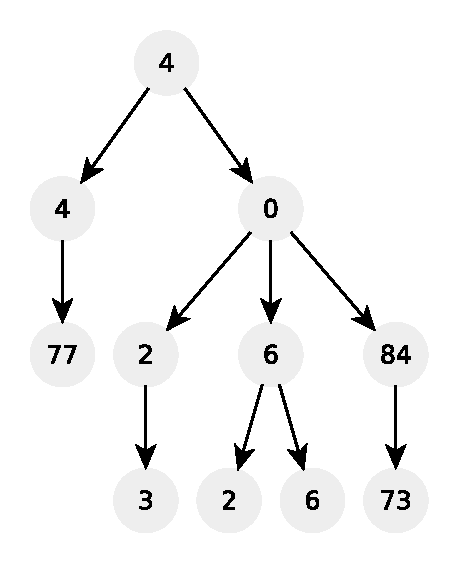
\includegraphics[width=1\linewidth]{sources/verify_BST/images/generic_tree}
		\caption[]{Example of a generic tree.}
		\label{fig:verify:generic_tree}
	 \end{subfigure}
	\hfill
	\begin{subfigure}[t]{0.46\textwidth}
		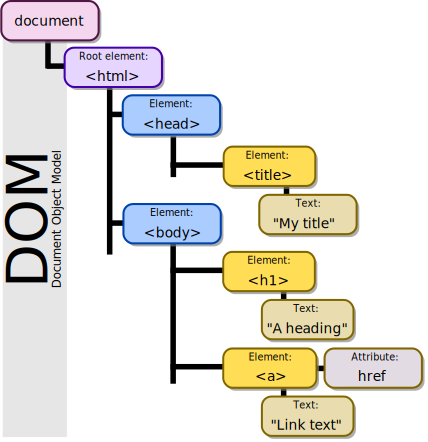
\includegraphics[width=1\linewidth]{sources/verify_BST/images/DOM-model}
		\caption[]{Example of DOM in a HTML document.}
		\label{fig:verify:DOM}}
	 \end{subfigure}
	 \caption[]{}
	  \label{fig:verify:trees}
\end{figure}



Binary search trees are a special kind of trees that are extremely useful when we need to arrange data on which the following operations need to be performed
\begin{itemize}
	\item insert
	\item delete
	\item search
	\item ceil/floor
\end{itemize}.
In this chapter we are going to look at a common interview question in which we will have to determine whether a given tree is a binary search tree or not. 

This classic problem should be really well understood as the structure of and the insights behind it solutions can be applied to many others binary tree problems.

\section{Problem statement}
\begin{exercise}
Given a binary tree \cite{cit:wiki:BST}, determine if it is a valid binary search tree (BST) which is defined as follows:
\begin{itemize}
    \item The left subtree of a node contains only nodes with keys less than the node's key.
    \item The right subtree of a node contains only nodes with keys greater than the node's key.
\end{itemize}
You can assume the function receives a pointer or a reference to a structure name \inline{TreeNode} which defined is shown in Listing \ref{list:verify_BST:tree_structure}. 

\end{exercise}

\begin{lstlisting}[language=c++, caption=Binary tree definition used in this exercice.,label=list:verify_BST:tree_structure]

 struct TreeNode {
     int val;
     TreeNode *left;
     TreeNode *right;
     TreeNode(int x) : val(x), left(nullptr), right(nullptr) {}
 };
 \end{lstlisting}


\begin{example}
	\label{example:verify_BST:example1}
	\hfill \\
	For the tree shown in Figure \ref{fig:verify:example1} the function should return \textbf{false}.
	
\end{example}

\begin{example}
	\label{example:verify_BST:example3}
	\hfill \\
	For the tree shown in Figure \ref{fig:verify:example3} the function should return \textbf{true}.
	
\end{example}

\begin{example}
\label{example:verify_BST:example4}
	\hfill \\
	For the tree shown in Figure \ref{fig:verify:example4} the function should return \textbf{true}.

\end{example}


\begin{figure}
	\vspace*{-0.5in}
	\centering
	\begin{subfigure}[t]{0.30\textwidth}
		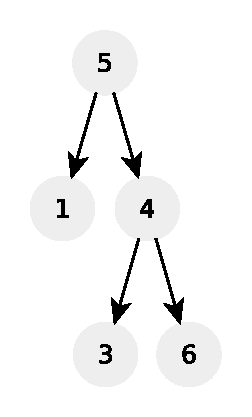
\includegraphics[width=1\linewidth]{sources/verify_BST/images/example1}
		\caption[]{Tree in Example \ref{example:verify_BST:example1}}
		\label{fig:verify:example1}
	 \end{subfigure}
	\hfill
	\begin{subfigure}[t]{0.30\textwidth}
		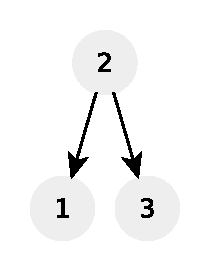
\includegraphics[width=1\linewidth]{sources/verify_BST/images/example3}
		\caption[]{Tree in Example \ref{example:verify_BST:example3}}
		\label{fig:verify:example3}
	 \end{subfigure}
	 \hfill
	 \begin{subfigure}[t]{0.30\textwidth}
		 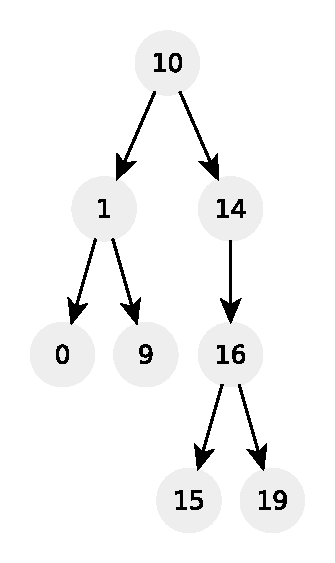
\includegraphics[width=1\linewidth]{sources/verify_BST/images/example4}
		 \caption[]{Tree in Example \ref{example:verify_BST:example4}}
		 \label{fig:verify:example4}
	  \end{subfigure}
	 \caption[]{}
	  \label{fig:verify:trees}
\end{figure}



\section{Clarification Questions}

\begin{QandA}
	\item Are all elements in the tree distinct?
	\begin{answered}
		\textit{Yes, you can assume all elemets are distinct.}
	\end{answered}
	\item How many nodes does the tree contain?
	\begin{answered}
		\textit{Up to $10^6$ nodes.}
	\end{answered}
\end{QandA}

\section{Discussion}
\label{verify_BST:sec:discussion}
The question is asking for a function that verifies whether a given tree is a binary search tree or not. But what does it mean exactly?
A tree $T$ is a binary search tree if:
\begin{enumerate}
	\item Every node has two subtree (named left and right, respectively) i.e. $T$ is a binary tree
	\item given a node $n$ in the tree \textbf{all} the nodes in its left subtree are smaller than the value in $n$.
	\item additionally,  \textbf{all} nodes in the right subtree are larger.
\end{enumerate}
For instance the tree in Figure \ref{ex:verify_BST:no_BST} is not a valid BST because node $15$ is a right descendent of the root but is it not greater than it. 

\begin{figure}
	\centering
	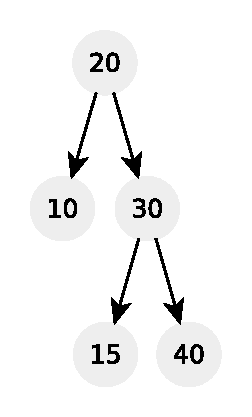
\includegraphics[width=0.3\linewidth]{sources/verify_BST/images/no_BST}
	\caption{Example of a binary tree that is not a BST.}
	\label{ex:verify_BST:no_BST}
\end{figure}



\subsection{A common mistake}
When solving this question a very common mistake is to use the following greedy algorithm to verify the BST property: for each node $n$ of the tree verify that \lstinline[columns=fixed]{n.val > n->left.val && n.val < n->right.val} i.e. that the value of the node curreclty analyzed is greater than the value of its left child but smaller than its right one. This algorithm might work even for some trees but fails on others, and it is thus not correct. For instance the algorithm described above fails on the example \ref{ex:verify_BST:no_BST} as it will say that it is a valid BST.

It is clear at this point that all nodes in the tree need to be visited in order to verify whether the BST property holds and that somehow the information about the values from nodes higher in the tree need to be passed down to the children and descendants. Let's see how this can be done.

\subsection{Top Down approach}
\label{verify_BST:sec:topdown}
When talking about tree, one should immediately think about a top down approach and recursion. This problem is no different and in-fact  becomes almost trivial if approached using recursione and the following key considerations are made:
\begin{enumerate}
	\item every node can be thought as the root of a tree for which the BST property needs to hold (and thus verified). 
	\item empty trees satisfy the BST property
	\item every nodes must be within a certain range that is determined by its parent. For instance, given the node $15$ in the example \ref{example:verify_BST_:one}, in order for the tree to be a valid it must be within the range $(14,16)$. Why is that? Because its parent, the node $16$ must be within the range $(14,+\infty)$ and additionally node $15$, being the left subtree of node $16$ must be lower than its parent. The same reasoning can be applied recusively up to the root of the tree where the range of the value is simply $(-\infty, +\infty)$ (no constraints). 

	The node $9$ in the example \ref{example:verify_BST_:one} must be within the range $(1,10)$ for similar reasons.
\end{enumerate}


To summarize, we can visit the tree in a top-down fashion and maintain a range that the current node must satisfy starting with a range equal to $(-\infty, +\infty)$ for the root (meaning that de-facto there is no restriction on the value the root can take). Once the value is checked against the range, then the same function can be applied to the right and left children but making sure that the range is modified accordingly when recurring on the children. 

But how does such a range change when visiting down the tree? The idea is simple: Given a node $n$ with parent $p$ and range \( (l_p, u_p) \) then:
\begin{itemize}
	\item if $n$ is the right child of $p$, then the range for $n$ is: $(p, u_p)$: all nodes in the right subtree of $p$ must be \textbf{higher} than $p$. Note that $p > l_p$ (otherwise the BST property would be violeted when checking $p$) and thus the range for $n$ becomes smaller meaning that all the constrains coming from the ancestors of $p$ will also be satisfied with the new range $(p, u_p)$.
	\item A similar reasoning applies if $n$ is the left child of $p$. The range for $n$ is then : $(l_u,p)$.
\end{itemize}

The idea above is shown in Listing \ref{list:verify_BST}. Note how short and concise the code can be implemented with recursion.  The complexity of this approach is $O(n)$ time and $O(1)$ space (if you do not count the space on the stack taken by the recursion.
\lstinputlisting[language=c++, caption=Linear time recursive solution to the problem of verifying the BST property.,label=list:verify_BST]{sources/verify_BST/verify_BST_solution1.cpp}


\subsection{Brute force}
Another way to solve this problem is to read carefully the definition of BST and realize that, for each node $n$ we need to check if the left subtree contains any element greater than $n$ and whether its right subtree contains any element smaller than $n$. This problem becomes almost trivial provided two functions are available, \lstinline[columns=fixed]{min_tree(TreeNode* root)} and \lstinline[columns=fixed]{max_tree(TreeNode* root)} for retrieving the min and max value respectively of a tree. The idea above can be implemented as shown in Listing \ref{list:verify_BST_bruteforce}

\lstinputlisting[language=c++, caption=Quadratic solution to the problem of verifying the BST property.,label=list:verify_BST_rbuteforce]{sources/verify_BST/verify_BST_solution2.cpp}